\documentclass[11.5pt, aspectratio=169]{beamer}
\usepackage{amsmath, amssymb, stmaryrd, mathpartir, commath, url, longtable,hyperref,tabularx}

\usepackage{forloop, microtype}
\usepackage{wasysym}
%\usepackage[dvipsnames]{xcolor}
\usepackage{csquotes}
%\usepackage{mathptmx}
\usepackage{listings}
\hypersetup{colorlinks=true,citecolor=blue}
\RequirePackage{subcaption}
\captionsetup{compatibility=false}
\usepackage{graphicx}
\usepackage{xspace}
\usepackage{dirtytalk}
\usepackage{xparse}% http://ctan.org/pkg/xparse
\usepackage{etoolbox}% http://ctan.org/pkg/etoolbox
\usepackage{tikz}
\newcommand{\lambdacalc}{\ensuremath{\lambda}-calculus\xspace}
\newenvironment{fake}[1]{\par\vspace{3pt}\noindent\textbf{#1}\itshape}{\normalfont\ignorespacesafterend\vspace{3pt}\par}

\usepackage{float}
\floatstyle{boxed}
\restylefloat{figure}
\usepackage{verbatim}

\newcommand{\backupbegin}{
   \newcounter{finalframe}
   \setcounter{finalframe}{\value{framenumber}}
}
\newcommand{\backupend}{
   \setcounter{framenumber}{\value{finalframe}}
}

\setbeamercovered{%
  again covered={\opaqueness<1->{15}}}



% TIKZ STUFF

\tikzstyle{arrow} = [thick,->]
\tikzstyle{diagnode} = [rectangle, rounded corners, minimum width=5cm, minimum
height=1cm,text centered, text width=5cm, draw=black, anchor=center, fill=red!30]


\usepackage{amsmath,verbatim}

\lstdefinelanguage{Links}{%
  morekeywords={typename, fun, linfun, op, var, if, this, true, false, else, case, switch, handle,
    handler, shallowhandler, open, do, sig, new, send, receive, spawnAt, spawn,
module, request, accept, try, as, in, otherwise, catch, offer, select, raise,
fork, spawnClient, cancel, catch, for, where},%
  sensitive=t, %
  comment=[l]{\#\ },%
  escapeinside={(*}{*)},%
  morestring=[d]{"},%
  keywordstyle=\color{blue},
  showstringspaces=false
  %frame = single
 }

% Links style
\lstset{
  basicstyle=\linespread{1.3}\ttfamily\large,
  keywordstyle=\bfseries,
  language=Links,
  backgroundcolor=\color{white}
}


\usepackage{expl3,xparse}
\makeatletter
\let\old@lstKV@SwitchCases\lstKV@SwitchCases
\def\lstKV@SwitchCases#1#2#3{}
\makeatother
\usepackage{lstlinebgrd}
\makeatletter
\let\lstKV@SwitchCases\old@lstKV@SwitchCases

\lst@Key{numbers}{none}{%
    \def\lst@PlaceNumber{\lst@linebgrd}%
    \lstKV@SwitchCases{#1}%
    {none:\\%
     left:\def\lst@PlaceNumber{\llap{\normalfont
                \lst@numberstyle{\thelstnumber}\kern\lst@numbersep}\lst@linebgrd}\\%
     right:\def\lst@PlaceNumber{\rlap{\normalfont
                \kern\linewidth \kern\lst@numbersep
                \lst@numberstyle{\thelstnumber}}\lst@linebgrd}%
    }{\PackageError{Listings}{Numbers #1 unknown}\@ehc}}
\makeatother

\ExplSyntaxOn
\NewDocumentCommand \lstcolorlines { O{green} m }
{
  \clist_if_in:nVTF { #2 } { \the\value{lstnumber} }{ \color{#1} }{\color{white}}
}
\ExplSyntaxOff
\newcommand{\textl}{\text{\lightning}}


\newcommand{\calcwd}[1]{\mathbf{\mathbf{#1}}}
\newcommand{\one}{\mathbf{1}}
\newcommand{\lightningnu}[1]{\nu #1\lightning}
\newcommand{\gvqueue}[4]{#1(#2){\leftrightsquigarrow} #3(#4)}
\newcommand{\mkwd}[1]{\ensuremath{\mathsf{#1}}}
\newcommand{\gvsend}[2]{\calcwd{send} \: #1 \: #2}
\newcommand{\gvrecv}[1]{\calcwd{receive} \: #1}
\newcommand{\gvcancel}[1]{\calcwd{cancel} \app #1}
\newcommand{\gvclose}[1]{\calcwd{close} \app #1}
\newcommand{\gvcancelup}[1]{\calcwd{cancel} \app #1}
\newcommand{\gvout}[2]{!{#1}.{#2}}
\newcommand{\gvin}[2]{?{#1}.{#2}}
\newcommand{\gvend}{\mathsf{End}\xspace}
\newcommand{\gvfork}[1]{\calcwd{fork} \, #1}
\newcommand{\app}{\:}
\newcommand{\inl}[1]{\calcwd{inl} \app #1}
\newcommand{\inr}[1]{\calcwd{inr} \app #1}
\newcommand{\gvcase}[2]{\calcwd{case} \: #1 \: \calcwd{of} \: \{ #2 \}  }
\newcommand{\gvlet}[3]{\calcwd{let} \: #1 = #2 \: \calcwd{in} \: #3}
\newcommand{\tryasinotherwise}[4]{\calcwd{try} \: #1 \: \calcwd{as} \: #2 \: \calcwd{in} \: #3 \: \calcwd{otherwise} \: #4}
\newcommand{\raiseexn}{\calcwd{raise}\xspace}
\newcommand{\un}[1]{\mkwd{un}(#1)}
\newcommand{\gvdual}[1]{\overline{#1}}
%\newcommand{\compat}{\asymp}
\newcommand{\evalperhaps}{\eval^?}
\newcommand{\evalstar}{\eval^*}
\newcommand{\scancel}[1]{\text{\lightning} #1}
\newcommand{\scancelmv}[1]{#1 \lightning}
\newcommand{\config}[1]{\mathcal{#1}}
\newcommand{\seq}[1]{\overrightarrow{#1}}
\newcommand{\fv}[1]{\mathsf{fv}(#1)}
%\newcommand{\fcv}[1]{\mathsf{fcv}(#1)}
\newcommand{\fvs}[1]{\mathsf{fvs}(#1)}
\newcommand{\fn}[1]{\mathsf{fn}(#1)}
\newcommand{\fcvs}[1]{\fn{#1}}
\newcommand{\chansharp}[1]{#1^{\sharp}}
\newcommand{\chanflat}[1]{#1^{\flat}}
\newcommand{\without}{/}
\newcommand{\equivceval}{\equiv \longrightarrow_{\textsf{C}} \equiv}
\newcommand{\cevalthick}{\Longrightarrow_{\textsf{C}}}
\newcommand{\ceval}{\quad \longrightarrow \quad}
\newcommand{\teval}{\longrightarrow_{\textsf{M}}}
\newcommand{\eps}[1]{\mkwd{eps}(#1)}
\newcommand{\affected}[1]{\mkwd{affected}(#1)}
\newcommand{\halt}{\calcwd{halt}\xspace}
\newcommand{\bcirc}{\bullet}
\newcommand{\wcirc}{\circ}
\newcommand{\disable}[1]{\mkwd{disable}(#1)}

\newcommand{\blocked}[2]{\mkwd{blocked}(#1, #2)}
\newcommand{\depends}[3]{\mkwd{depends}(#1, #2, #3)}
\newcommand{\deadlocked}[1]{\mkwd{deadlocked}(#1)}

\newcommand{\Ceval}{\Longrightarrow_{\textsf{C}}}

\newcommand{\dom}[1]{\mkwd{dom}(#1)}

\newenvironment{remark}{\paragraph{Remark.}}{\hfill \tiny{$\square$}}
%\newtheorem{remark}{Remark}
%\newtheorem{lemma}{Lemma}
%\newtheorem{proposition}{Proposition}
%\newtheorem{corollary}{Corollary}
%\newtheorem{definition}{Definition}


\newcommand{\defeq}{\triangleq}

\newcommand{\todo}[1]{{\noindent\small\color{red} \framebox{\parbox{\dimexpr\linewidth-2\fboxsep-2\fboxrule}{\textbf{TODO:} #1}}}}
\newenvironment{subcase}[1]
  {\textbf{Subcase #1} \hfill \\
  \begin{adjustwidth}{0.25cm}{}}
  {\end{adjustwidth}}

\newenvironment{proofcase}[1]
  {\totheleft{\textbf{Case \textsc{#1}}}}
  {}
\newcommand{\lto}{\multimap}
\newcommand{\proofstep}[1]{
  \begin{compactitem}
  \item #1
  \end{compactitem}
}

\newcommand{\names}[1]{\mkwd{names}(#1)}

\arraycolsep=1pt%\def\arraystretch{2.2}

\newcommand{\transl}[1]{\llbracket #1 \rrbracket}
\newcommand{\stranslateb}[1]{\mathcal{S}\llparenthesis #1 \rrparenthesis}
\newcommand{\ttranslateb}[1]{\mathcal{T}\llparenthesis #1 \rrparenthesis}
\newcommand{\etranslateb}[1]{\mathcal{E}\llparenthesis #1 \rrparenthesis}
\newcommand{\ptranslateb}[1]{\mathcal{P}\llparenthesis #1 \rrparenthesis}

\newcommand{\gvoutone}[1]{{!}#1}
\newcommand{\gvinone}[1]{{?}#1}
\newcommand{\letintwo}[2]{\calcwd{let} \: #1 = #2 \: \calcwd{in}}
\newcommand{\totheleft}[1]{\begin{flushleft}#1\end{flushleft}}
\usepackage[T1]{fontenc}
\usepackage[scaled=0.85]{beramono}
\newcommand\doubleplus{+\kern-1.3ex+\kern0.8ex}
\newcommand{\metadef}[1]{\calcwd{#1}}


\newcommand{\runtimechan}[2]{\mkwd{Channel}(#1, #2)}
\newcommand{\closure}[2]{\langle #1, #2 \rangle}
%\newcommand{\boldleft}{\textbf{\{ }}
%\newcommand{\boldright}{\textbf{ \}}}
\newcommand{\contained}[1]{\metadef{Channels}(#1)}

\newcommand{\ba}{\begin{array}}
\newcommand{\ea}{\end{array}}

\newcommand{\bl}{\ba[t]{@{}l@{}}}
\newcommand{\el}{\ea}


\newcommand{\triestosend}[4]{{#1} \xRightarrow[#4]{#2} {#3}}

\newcommand{\notsmall}{}

\newcommand{\oftype}{\,{:}\,}

\newcommand{\sendpair}[2]{\calcwd{send} \: (#1, #2)}

%\renewcommand{\paragraph}[1]{\textbf{\textit{#1}}}
\usepackage{tikz-cd}

\newcommand{\exnty}{\mkwd{Exn}\xspace}
\newcommand{\raiseexnP}[1]{\calcwd{raise} \: #1}
\newcommand{\tryinunless}[4]{\calcwd{try} \: #1 \: \calcwd{as} \: #2 \:
    \calcwd{in} \: #3 \: \calcwd{unless} \: #4}

\newcommand{\handled}[1]{\mkwd{Handled}(#1)}

\newcommand{\highlight}[1]{{\color{colorredorange} #1} }
\newcommand{\highlightpink}[1]{{\color{colorpink} #1} }
\newcommand{\highlightwarning}[1]{{\color{colorlightpink} #1} }
\newcommand{\midspace}{\; \mid{} \; }
\setlength\tabcolsep{1.5em}

\newcommand{\lact}{\lambda_{\text{act}}\xspace}
\newcommand{\lch}{\lambda_{\text{ch}}\xspace}

\usepackage{config/presento}
\usepackage{framed}
\usepackage{stmaryrd}
\usepackage{amsmath}
\usepackage{wasysym}
% Presento style file
\usepackage{float,lipsum}
\floatstyle{boxed}
\usepackage{mathpartir}
% custom command and packages
% custom packages
\usepackage{textpos}
\setlength{\TPHorizModule}{1cm}
\setlength{\TPVertModule}{1cm}

\newcommand\crule[1][black]{\textcolor{#1}{\rule{2cm}{2cm}}}


\usepackage{verbatim}
% Information
\title{Cross-tier web programming for curated databases: A case study}
\author{Simon Fowler$^1$, Simon D.\ Harding$^1$, Joanna, Sharman$^2$, James Cheney$^1$}
\institute{University of Edinburgh$^1$\\
  Novo Nordisk$^2$}
\date{19th February 2020}

\begin{document}

% Title page
\begin{frame}[plain]
\titlepage


\hfill
\vspace{-1em}
$
\renewcommand*{\arraystretch}{1.8}
\begin{array}{r}
   
\includegraphics[height=0.7cm, keepaspectratio]{images/logos/inf_uoe.png} \\
   
\includegraphics[height=1.25cm,
   keepaspectratio]{images/logos/erc-logo.jpg} \\
\end{array}
$
\end{frame}


\begin{frame}{Curated Scientific Databases}

  \begin{fullpageitemize}
  \item {\LARGE \textbf{Curated Databases:}}
    \begin{itemize}
      \itemR ``databases that are populated and updated with a great deal of human effort'' (Buneman et al., 2008)
      \itemR Examples: CIA World Factbook, GtoPdb
    \end{itemize}
    \vspace{1em}
  \item {\LARGE \textbf{Curation challenges:}}
    \begin{itemize}
      \itemR Annotation propagation, provenance
        tracking, citation, archiving\ldots
      \itemR Have to be hand-crafted for every curated DB ---
        often with very stretched resources
    \end{itemize}
    \vspace{1em}
  \item {\LARGE \textbf{Ultimate goal: programming
      language support for curation
  functionality}}
    \begin{itemize}
      \itemR Previous work (Fehrenbach \& Cheney, 2018) has already added
        provenance tracking!
    \end{itemize}
  \end{fullpageitemize}
\end{frame}

\begin{frame}{Cross-tier web programming}

  \begin{center}
    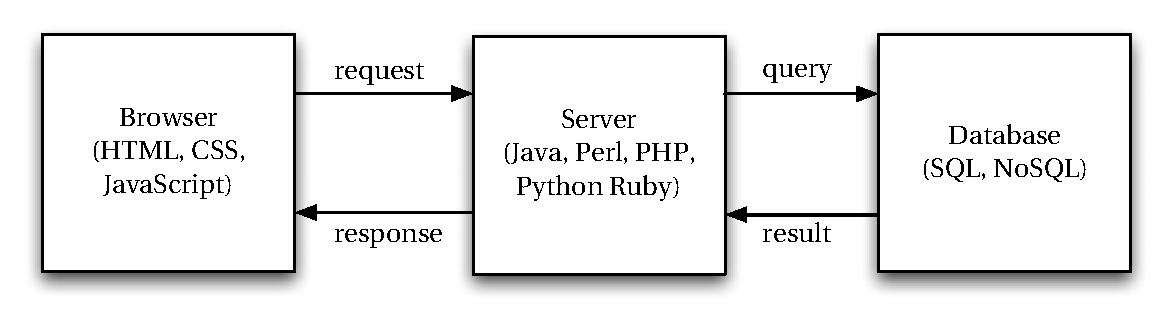
\includegraphics[width=0.75\textwidth]{images/3tier.pdf}
  \end{center}

  \begin{fullpageitemize}
  \item Curated databases normally a
    \emph{collection of applications}:
    \begin{itemize}
      \itemR Database, web frontend, curation application
    \end{itemize}
    \vspace{1em}
  \item \textbf{Cross-tier} programming languages:
    \begin{itemize}
      \itemR Client, server, and database code written in same language
      \itemR \textbf{Links}: research cross-tier programming language developed
        at UoE since 2006
    \end{itemize}
    \vspace{1em}
  \item Before considering curation support, \emph{can cross-tier programming
    languages handle a real-world case study?}
  \end{fullpageitemize}
\end{frame}


\begin{frame}{GtoPdb: IUPHAR/BPS Guide to PHARMACOLOGY}
  \begin{minipage}{0.525\textwidth}
    \begin{fullpageitemize}
    \item Popular curated database detailing around 3000 pharmacological targets (e.g.,
      receptors) and 9700 ligands (e.g., drugs)
      \vspace{1em}
    \item Initially IUPHAR-DB, started in 2003
      \vspace{1em}
    \item Manually updated by curation team at
      UoE, on advice of subcommittees
      \vspace{1em}
    \item Written in Java. Scale (as of late 2019):
      \begin{itemize}
        \itemR \emph{89MB} of data in \emph{181 tables}
        \itemR \emph{17935 lines} of data transformation code
        \itemR \emph{28819 lines} of JSP rendering code
        \itemR \emph{43129 lines} of data access code
      \end{itemize}
    \end{fullpageitemize}
  \end{minipage}
  \hfill
  \begin{minipage}{0.4\textwidth}
    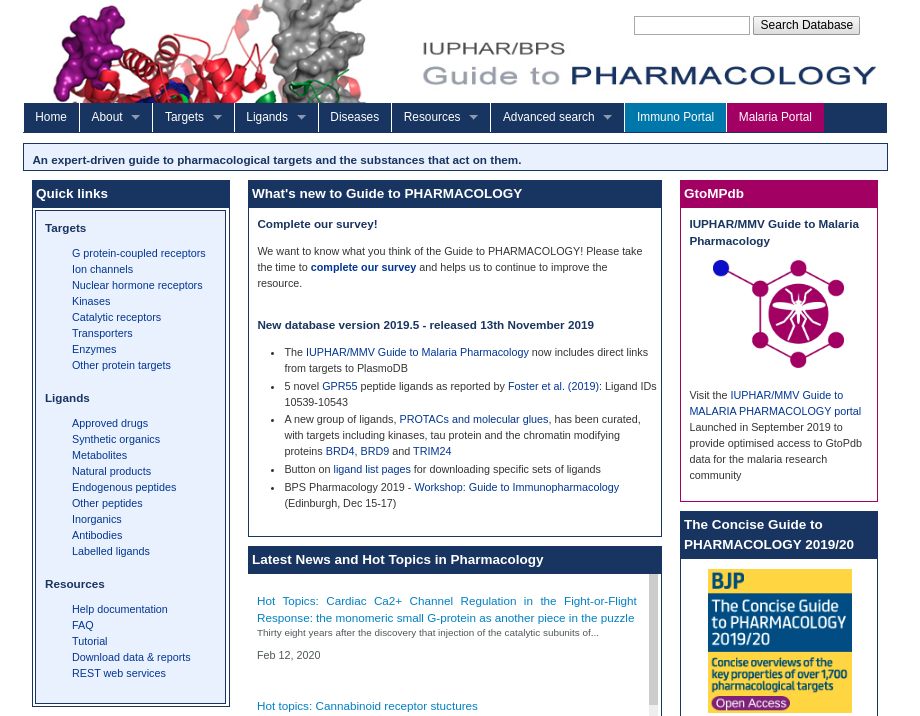
\includegraphics[width=\textwidth]{images/gtopdb-screenshot.png}
  \end{minipage}

\end{frame}

\framecard{{\color{white}\bigtext{Implementing GtoPdb in Links}}}

\begin{frame}[fragile]{GtoPdb Page Lifecycle}

  \begin{minipage}{0.3\textwidth}
     % TODO: Diagram (TiKZ?)
    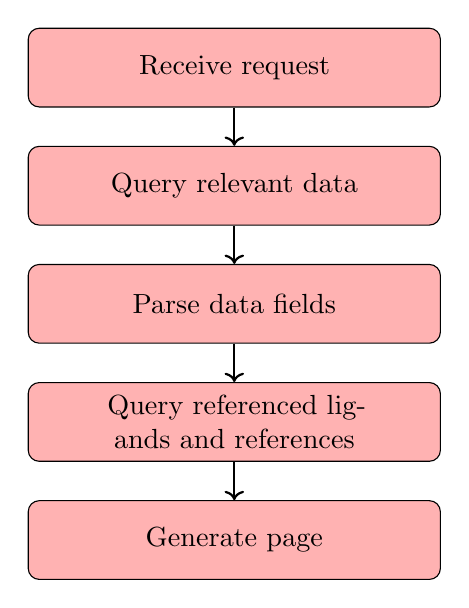
\begin{tikzpicture}[node distance=1.5cm]
      \node (0) [diagnode] { Receive request };
      \node (1) [diagnode, below of=0]{ Query relevant data };
      \node (2) [diagnode, below of=1]{ Parse data fields };
      \node (3) [diagnode, below of=2]{ Query referenced ligands and references };
      \node (4) [diagnode, below of=3]{ Generate page };

      \draw [arrow] (0) -- (1);
      \draw [arrow] (1) -- (2);
      \draw [arrow] (2) -- (3);
      \draw [arrow] (3) -- (4);
    \end{tikzpicture}
  \end{minipage}
  \hfill
  \begin{minipage}{0.575\textwidth}
    {\small
      \begin{verbatim}
Some substituted benzazepines such as SKF-83959
are G-protein biased agonists of the dopamine
D<sub>1</sub> receptor and fail to activate
&beta;-arrestin recruitment <Reference id=28036/>;
their ability to signal through
G<sub>q</sub>-mediated pathways has been
controversial <Reference id=33435/>.
\end{verbatim}
  }

  \begin{center}
    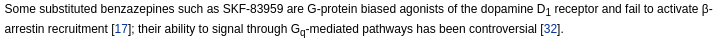
\includegraphics[width=1.075\textwidth]{images/rendered.png}
  \end{center}
  \end{minipage}


\end{frame}

\begin{frame}[fragile]{Language-Integrated Query}

  \begin{minipage}[t]{0.45\textwidth}
    {\large \textbf{SQL}}
    \begin{lstlisting}[language=sql]
SELECT name FROM ligand
WHERE approved
    \end{lstlisting}
  \end{minipage}
  %
  \hfill
  %
  \begin{minipage}[t]{0.45\textwidth}
    {\large \textbf{Links}}
    \begin{lstlisting}[language=Links]
for (l <-- ligand)
  where (l.approved)
  [ l.name ]
    \end{lstlisting}
  \end{minipage}

  \begin{fullpageitemize}
  \item {\Large \emph{Language-integrated Query:}}
    \begin{itemize}
      \itemR Allow database queries to be written in host language, rather than SQL
    \end{itemize}
    \vspace{1em}
    \item { \Large \emph{Benefits}:}
    \begin{itemize}
      \itemR Full static typechecking of queries
      \itemR Only one language to learn
      \itemR Abstraction: parts of queries can be reused
    \end{itemize}
  \end{fullpageitemize}
\end{frame}

\begin{frame}[fragile]{Nested Queries}

  \begin{lstlisting}[language=Links]
for ( l <-- ligand )
  [( name = l.name,
     synonyms =
       for ( l2s <-- ligand2synonym )
         where ( l2s.ligand_id == l.ligand_id )
         [ l2s.synonym ]
  )]
  \end{lstlisting}

  \begin{fullpageitemize}
    \item Links queries need not be flat: can have arbitrarily-nested collections
    \item \emph{Extensively} used in GtoPdb case study
    \item \emph{Static bound on query count}: number of collection types appearing in output
  \end{fullpageitemize}

\end{frame}

\framecard{{\color{white}\bigtext{Evaluation}}}

\begin{frame}{Methodology}

  \begin{fullpageitemize}
  \item<1->{\Large \textbf{Query count} }
    \begin{itemize}
      \itemR Number of queries performed per page load
      \itemR \emph{Expectation}: Links lower due to static query bounds
    \end{itemize}
    \vspace{1em}
  \item<2->{\Large \textbf{Query handling time} }
    \begin{itemize}
      \itemR Time taken to execute query and process results into data
        structures
      \itemR \emph{Expectation}: Either Links performs better due to fewer queries, or
        Java performs better due to faster marshalling
    \end{itemize}
    \vspace{1em}
  \item<3->{\Large \textbf{Page build time} }
    \begin{itemize}
      \itemR Time between request handler invocation and response being ready
%     \itemR Useful to consider both including \emph{and} excluding query
%       handling time
      \itemR \emph{Expectation}: Java to perform better due to JIT and maturity
    \end{itemize}
  \end{fullpageitemize}
    \vspace{1em}

    \onslide<4->{
  Performance measurements performed locally, using an instrumented Links
  interpreter and modified GtoPdb code. Sample of 150 random pages from
  object data and disease data pages.
}
\end{frame}

\begin{frame}{Query Count}

  \begin{minipage}[t]{0.45\textwidth}
    \centering
    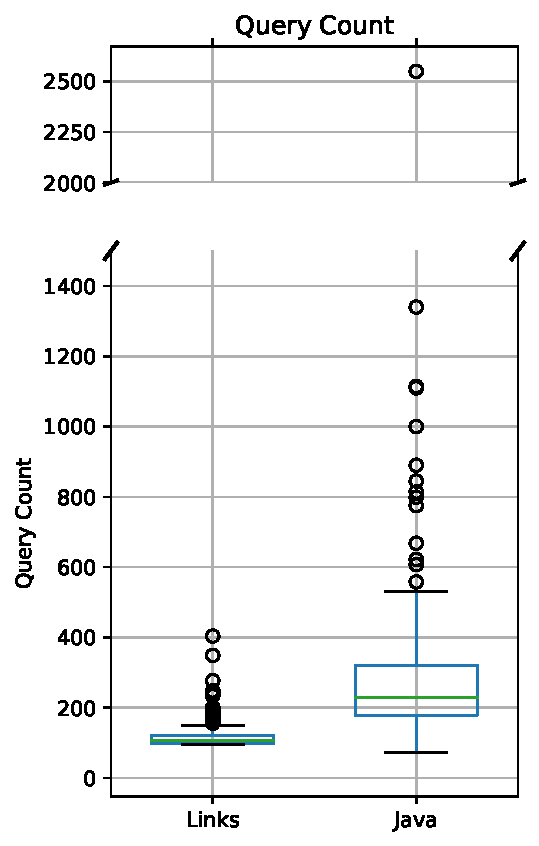
\includegraphics[scale=0.4]{images/objectdisplay_querycount_box.pdf}

    \begin{center}
      Object data page
    \end{center}
  \end{minipage}
  \hfill
  \begin{minipage}[t]{0.45\textwidth}
    \centering
    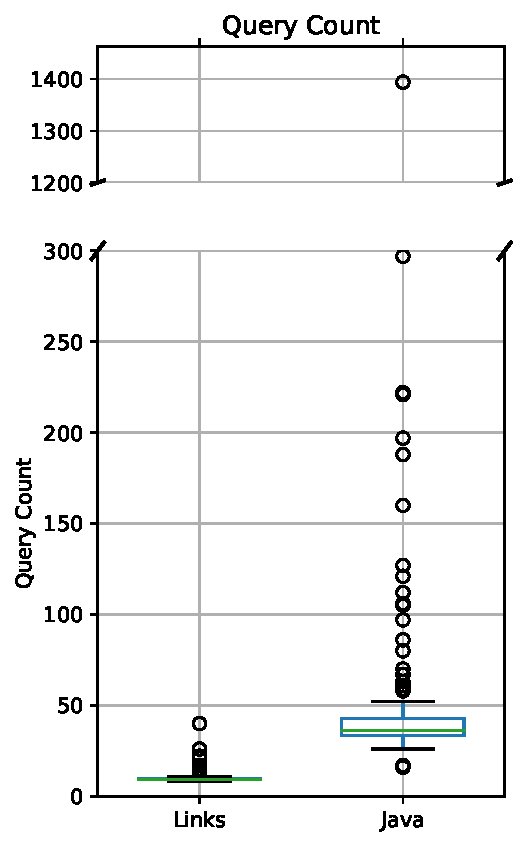
\includegraphics[scale=0.4]{images/diseasedisplay_querycount_box.pdf}

    \begin{center}
      Disease data page
    \end{center}
  \end{minipage}
  \vspace{1em}

  \begin{fullpageitemize}
  \itemR As expected, Links query count lower and more predictable
  \end{fullpageitemize}
\end{frame}

\begin{frame}{Query Handling Time}

  \begin{minipage}[t]{0.45\textwidth}
    \centering
    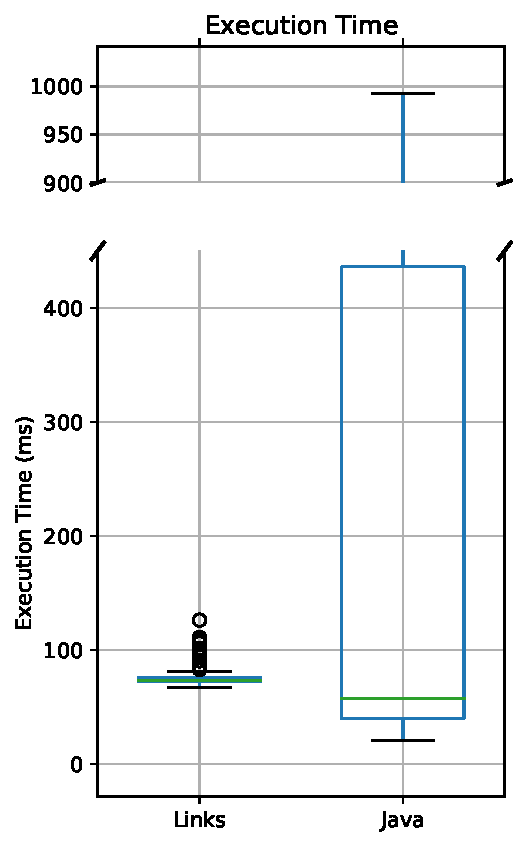
\includegraphics[scale=0.4]{images/objectdisplay_querytime_box.pdf}

    \begin{center}
      Object data page
    \end{center}
  \end{minipage}
  \hfill
  \begin{minipage}[t]{0.45\textwidth}
    \centering
    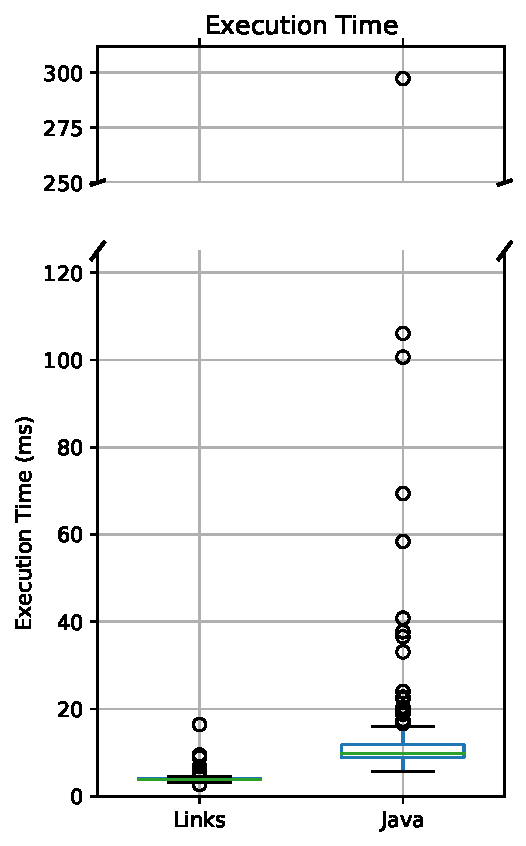
\includegraphics[scale=0.4]{images/diseasedisplay_querytime_box.pdf}

    \begin{center}
      Disease data page
    \end{center}
  \end{minipage}
  \vspace{1em}

  \begin{fullpageitemize}
  \itemR Links far more predictable due to more predictable query counts
  \itemR Median query time slightly higher on object display page, likely due to marshalling
  \end{fullpageitemize}
\end{frame}

\begin{frame}{Page Build Time}

\begin{minipage}[t]{0.45\textwidth}
    \centering
    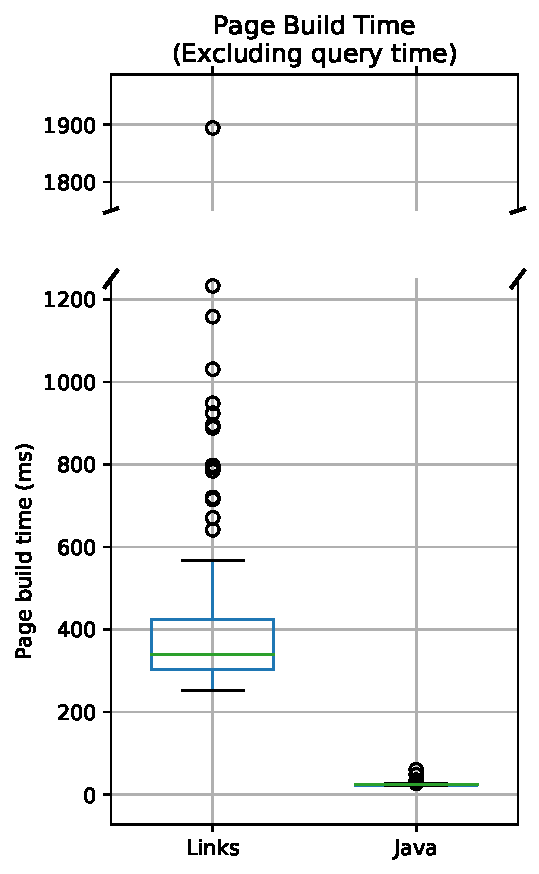
\includegraphics[scale=0.3]{images/objectdisplay_pagebuild_excl_box.pdf}
    ~
    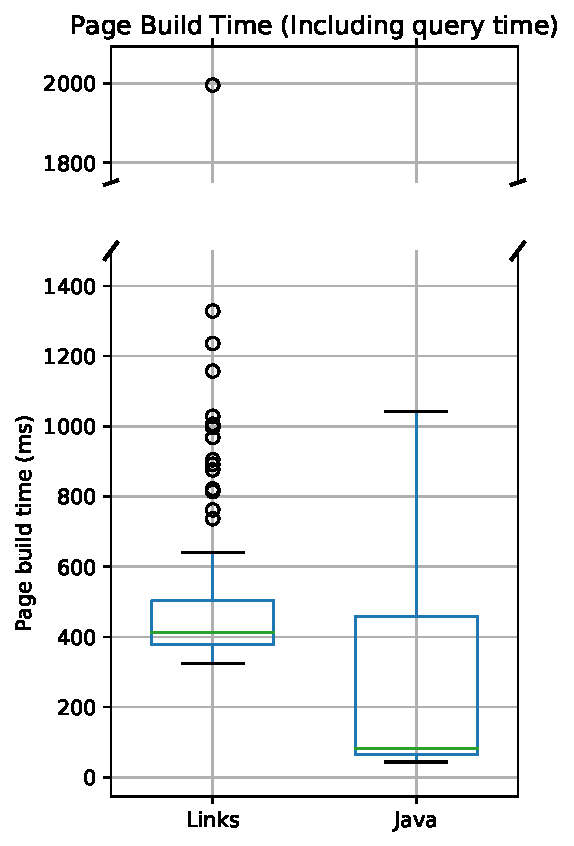
\includegraphics[scale=0.3]{images/objectdisplay_pagebuild_incl_box.pdf}

    \begin{center}
      Object data page
    \end{center}
  \end{minipage}
  \hfill
  \begin{minipage}[t]{0.45\textwidth}
    \centering
    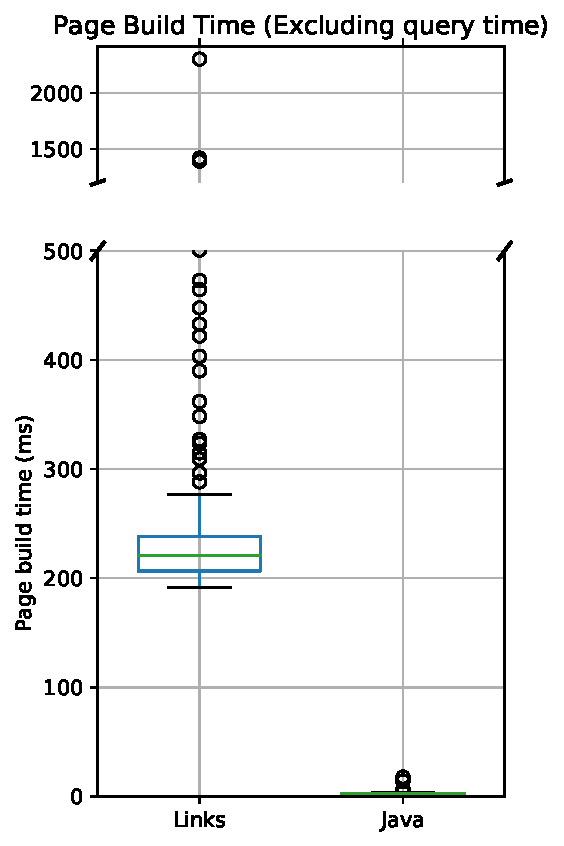
\includegraphics[scale=0.3]{images/diseasedisplay_pagebuild_excl_box.pdf}
    ~
    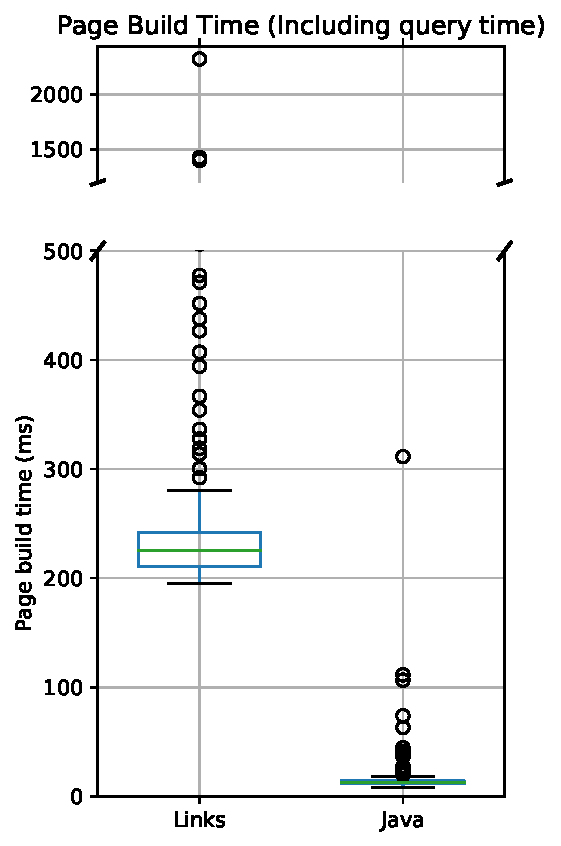
\includegraphics[scale=0.3]{images/diseasedisplay_pagebuild_incl_box.pdf}

    \begin{center}
      Disease data page
    \end{center}
  \end{minipage}
  \vspace{1em}

  \begin{fullpageitemize}
  \itemR As expected, Java page generation \emph{much} faster due to maturity
  \itemR Outliers in Links due to (slow) parsing of data fields for large pages
  \end{fullpageitemize}
\end{frame}

\begin{frame}{Disease and Ligand Lists}

  \centering
  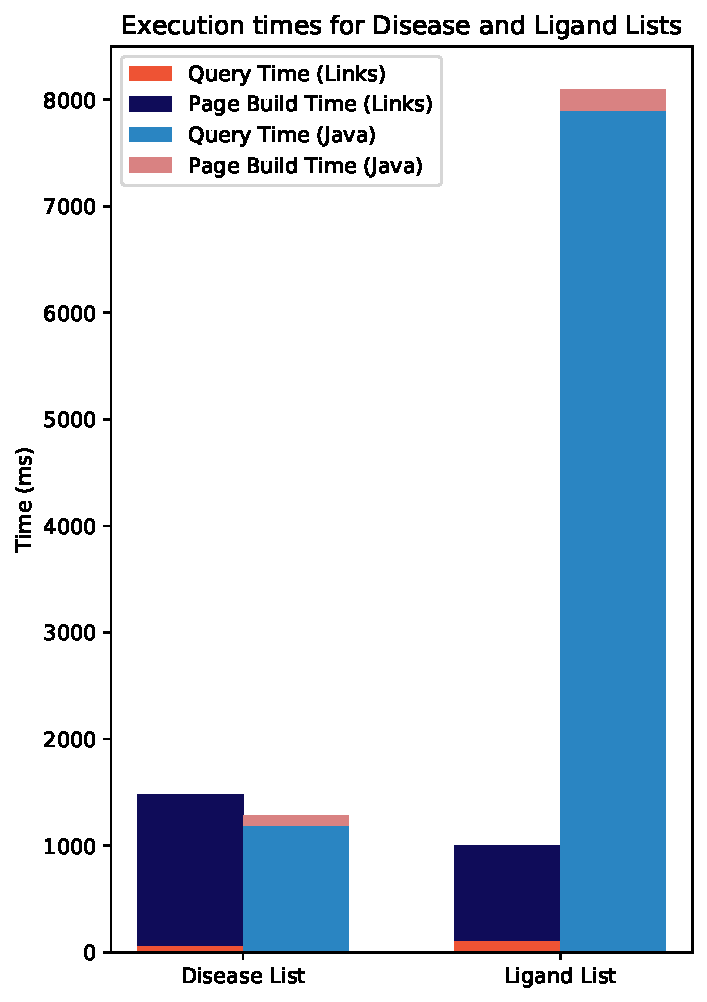
\includegraphics[scale=0.3]{images/diseaselist_stacked.pdf}
  \vspace{1em}

  \begin{fullpageitemize}
  \itemR List of all diseases and ligands
  \itemR Query counts in Java: 8995 (disease list) and 30479 (ligand list)
  \itemR \emph{Query counts in Links: 2!}
    \begin{itemize}
      \itemR \emph{Much} lower in Links due to nested queries \& no ORM used
    \end{itemize}
  \end{fullpageitemize}

\end{frame}


\framecard{{\color{white}\bigtext{Wrapping Up}}}

\begin{frame}{Ongoing Work: Curation Interface}

  \begin{minipage}{0.45\textwidth}
  \begin{center}
    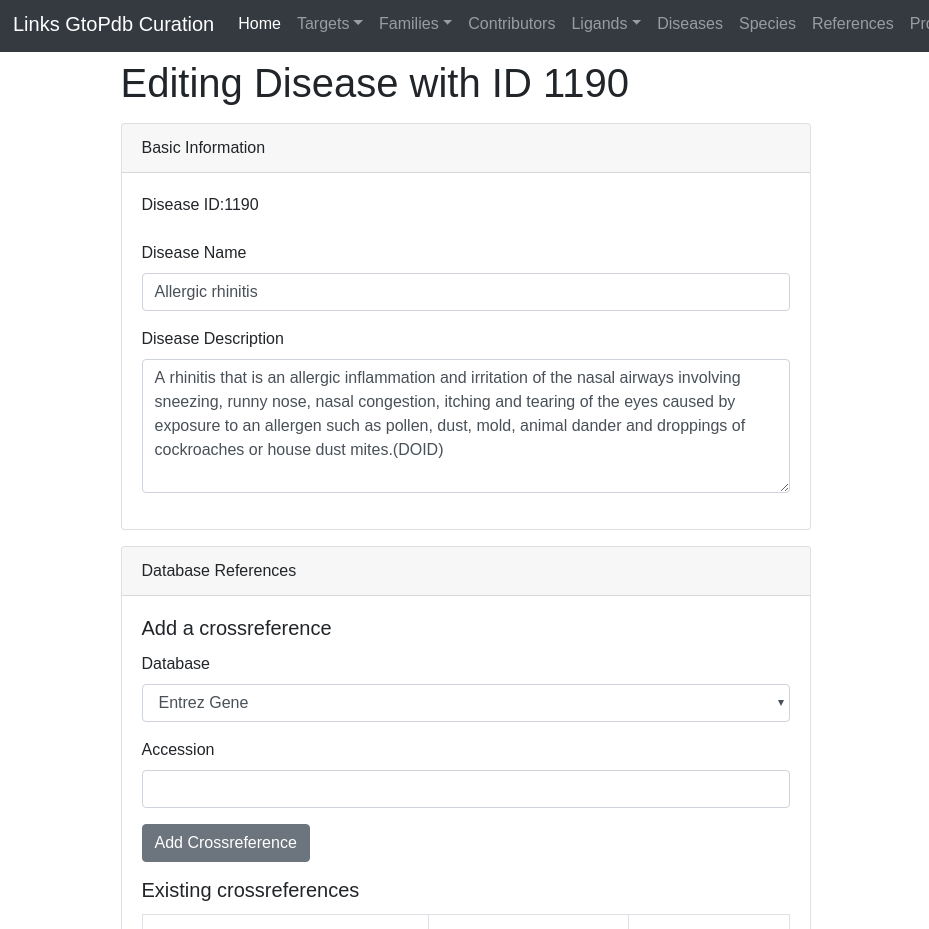
\includegraphics[width=\textwidth]{images/curation-interface.png}
  \end{center}
  \end{minipage}
  \hfill
  \begin{minipage}{0.5\textwidth}
  \begin{fullpageitemize}
  \item {\large \textbf{Ongoing work: Curation interface}}
    \begin{itemize}
      \itemR Implemented two illustrative pages from curation interface
      \itemR Aim to use these as realistic case study for curation functionality
    \end{itemize}
  \end{fullpageitemize}
\end{minipage}
\end{frame}

\begin{frame}[fragile]{Conclusion}

  \begin{fullpageitemize}
  \item {\LARGE \textbf{Summary}}
    \begin{itemize}
      \itemR \textbf{Curated databases}:
        \begin{itemize}
          \itemR Databases maintained using much human effort
          \itemR Consist of multiple applications: database, web
            frontend, curation interface
        \end{itemize}
%
      \itemR Cross-tier programming languages: client, server, database
        code in \emph{single language}
      \itemR First case study of reimplementing a large-scale curated database
        in a cross-tier programming language
      \itemR Performance results: Lower query counts; more predictable and often
        lower query times; but slower page build times
    \end{itemize}
  \end{fullpageitemize}

  {\large
  \begin{center}
    \verb+@Simon_JF+\\
    \verb+simon.fowler@ed.ac.uk+\\
    \url{http://www.links-lang.org}
  \end{center}
}
\end{frame}

\end{document}
